\chapter{Non-Volatile RAM}
\label{ch:nvram}

Conventional non-volatile memories such as HDD or SSD provide large capacities but are only block-oriented and incur substantial access latencies compared to volatile DRAM. Especially IO-bound applications tend to keep as much data in RAM as possible but are eventually forced to access slower media for durable storage. This led to the development of non-volatile variants of RAM. Recent research suggests that both fast and high-capacity NVRAM will become widely available in the near future.

This chapter gives an overview on the state-of-the-art in NVRAM research.
Included is a discussion of opportunities and challenges, such as the notorious
consistency issues in the presence of failures.

\section{Architectures and Applications}

There are numerous examples for applications of NVRAM. While earlier works often
considered NVRAM as a means to improve fault tolerance, recent research suggests
a broader range of applications. This development is especially driven by
recent advances in the manufacture of standalone NVRAM.

As pointed out earlier, a well-known use case of NVRAM is to increase fault
tolerance towards crashes. The goal is to retain main memory content even in
case of a crash, for instance by an abrupt power loss \cite{molina1992main,
eich1986main}. This way, critical data such as logs of file systems or databases
remain durable and can be used to recover and even complete unfinished
operations such as making a transaction durable \cite{liskov1991replication,
chen1996rio}. In the past, such solutions relied on battery-backed RAM. This was
subject to criticism as batteries only have a limited charge to ensure
durability. Also batteries degrade over time and need to be maintained to
prevent unexpected failure \cite{molina1992main}. Therefore, modern NVRAM
solutions which no longer require peripherals are a welcome improvement in this
area.

A significant amount of research on NVRAM is dedicated to mitigating the IO
bottleneck imposed by traditional disk storage. One way to do so is to defer
disk IO via durable disk caches \cite{chen1996rio, wu1994envy}. When an object
on disk is requested it is moved to the disk cache. Once an object is cached, it
may be read or modified without accessing the underlying disk. Write-back is
only required when there is not enough space for an incoming cache item. In
doing so, the number of data accesses involving disk IO can be greatly reduced.
Many operating systems including Linux or FreeBSD mimic this concept through the
use of page caches in volatile memory. The difference is that volatile caches
need to be flushed at some point which requires careful resource management.
NVRAM caches on the other hand, only need to evict items when there is no slot
for an incoming item.

Another approach is to treat NVRAM as an equivalent to traditional disk storage.
Early works, which were strongly influenced by the lack of high-capacity NVRAM,
proposed hybrid storage systems where disk storage was used in conjunction with
NVRAM \cite{wang2002conquest, miller2001hermes}. These works have very similar
assignment policies in that they only store small files such as metadata or
libraries in NVRAM whereas larger files remain on disk. While this does not
remove disk access as a common bottleneck, it certainly alleviates latency for
some frequently accessed files. In that regard, NVRAM-complemented disk storage
systems are similar to those with NVRAM disk caches.

For the time being, many applications will have to deal with a scarcity of
NVRAM. But as improving technologies achieve higher capacities with better
parameters, new system architectures become feasible. In some cases, traditional
storage may be eliminated altogether, making NVRAM the primary storage medium. A
prominent use case for this architecture are MMDB. These databases reside
entirely in main memory which drastically reduces latencies when accessing its
data. However, they are also vulnerable to crashes, as main memory is still
mostly volatile. In order to prevent data loss, MMDB have to mirror the entire
database to non-volatile memory. For that, they perform logging or checkpointing
to synchronize individual or groups of changes to non-volatile memory. When the
database is restarted, for example in response to a crash, checkpoints and
logging information are used to recover the most-recent state of the database
that was durable at the time of the crash. That is, MMDB require non-volatile
memory for the sole purpose of recovery. Recurring recovery measures such as
logging have been a long-standing issue with MMDB as they incur expensive disk
IO, thus limiting transaction throughput \cite{eich1986main, molina1992main,
wust2012efficient, malviya2014rethinking}. In addition, restarts reduce the
availability of a system as recovering large databases from slow storage can be
time-consuming. With NVRAM on the other hand, any MMDB would be implicitly
durable, hence making disk IO obsolete. Moreover, it has been shown that with
NVRAM logging is no longer necessary which paves the way for instantaneous
restarts \cite{oukid2015instant}. The concept of NVRAM-based MMDB is especially
promising as some upcoming variants of NVRAM are projected to feature larger
capacities than conventional DRAM \cite{lee2009architecting,
zilberberg2013phase, dulloor2014system}. For that reason, recent research has
investigated NVRAM-aware designs for MMDB ranging from KVS
\cite{bailey2013exploring, zhou2016nvht, wu2016nvmcached} to full-fledged
database systems \cite{oukid2015instant, schwalb2016hyrise, andrei2017sap}.
Research results in these areas are central to this work and are reflected in
chapter \ref{ch:nvram} through \ref{ch:concept}. Given their importance for this
thesis, existing KVS for NVRAM are looked into in more detail at the end of
chapter \ref{ch:kvs}.

While most works aim to improve existing architectures, some explore different
computation models. A recent example is a proposal to use NVRAM to enable
on-chip machine learning. The idea is to move away from the well-known Von
Neumann architecture and implement artificial neural networks by means of NVRAM
\cite{fumarola2016accelerating}. ANN perform a weighted sum over their inputs
before an activation function classifies the result. But before satisfiable
results can be obtained, ANN need to be trained by properly adjusting the scalar
weights of their inputs. It has been suggested that with NVRAM weight adjustment
could be performed on-chip where updated weights would be durable without the
need for write-back. However, neither artificial intelligence nor alternative
computation models are subject of this work.

Most proposals concerning NVRAM assume the presence of volatile RAM.
\cite{oukid2017data}. The reason behind this assumption is that not all parts of
memory may be intended for durability. Nonetheless, recent research suggests
that systems exclusively based on NVRAM can be built \cite{narayanan2012whole,
courtland2016can}. Clearly, such an architecture would have severe consequences
for both operating systems and applications \cite{bailey2011operating}. For
example, operating system processes would remain in memory even if terminated.
On the one hand, it could significantly accelerate the procedure of invoking a
process. On the other hand, all data belonging to a process' address space would
be durable even if they were corrupted by a crash. Other issues are concerned
about memory management, device drivers, and vital information. An early
prototype of such a system is currently in development \cite{courtland2016can}.
This topic however, is beyond the scope of this work and it is henceforth
assumed that volatile RAM will co-exist with NVRAM.

As shown above, NVRAM provides an opportunity to improve existing architectures
and even create new computation models. Given sufficient parameters such as
capacity and endurance, NVRAM could resolve the IO bottleneck of non-volatile
storage media. Especially systems such as MMDB have shown considerable gains in
transaction throughput and recovery times. Consequently, MMDB and in particular
KVS are at the center of this work.

\section{Technologies}

In the past, there have been multiple attempts to produce non-volatile
equivalents of main memory. One way is to emulate non-volatility by providing
backup power supplies or combining volatile DRAM and conventional non-volatile
storage in a single module. Another promising approach is to develop alternative
memory techniques that provide the features of NVRAM.

% This section presents notable developments in the field of NVRAM.

\todo[inline]{Present Phase-Change Memory (Concept/History/Parameters)}

% \paragraph{Early Approaches}
%
% Initially, the intention was to make systems more tolerant to failures, although
% opportunities for storage systems were also discussed \cite{molina1992main,
% wang2002conquest}. The main issue with DRAM is that, in order to retain its
% data, it needs to refresh its cells which requires a power supply. Therefore,
% early non-volatile main memories were equipped with batteries or UPS which
% allowed to hold information for a limited time in case of a power failure.
% Notable examples for systems using battery-backed DRAM are the file systems
% \emph{Harp} \cite{liskov1991replication} and \emph{Conquest}
% \cite{wang2002conquest} as well as the file cache \emph{Rio} \cite{chen1996rio}.
%
% In another approach, researchers used battery-backed SRAM as a write buffer
% which is flushed to an interconnected flash memory when full or in case of a
% power failure \cite{wu1994envy}. By limiting access to the SRAM, the
% non-volatile yet slower flash device is effectively shadowed. Still, since flash
% operates in block mode, the byte-addressable nature of SRAM cannot be exploited
% in this setup. This is an early example of hybrid memory solutions for fast mass
% storage. However, backup power supplies have also been subject to criticism.
% Arguments are that batteries are not inherently reliable and introduce
% additional maintenance overhead \cite{molina1992main}. Therefore experiments
% were conducted, where flash memory was directly attached to the memory interface
% \cite{shi2010write}. Similar ideas were later consolidated in the JEDEC NVDIMM
% specification, which defines several configurations for DIMMs consisting of
% flash memory and DRAM \cite{oe2016feasibility, huang2014design}.
%
% % This marks a shift in the development of NVRAM as reliability becomes second
% % to fast high-capacity storage.
%
% \paragraph{Modern Approaches}
%
% Early approaches for practical NVRAM were focused on making volatile DRAM retain its information across power outages. There are however promising alternatives such as PCM, MRAM or RRAM which are both byte-addressable and non-volatile by design. Although their underlying principles have been known for a while, further research was required to reach practical designs for manufacturing. Recent research suggests that these NVM technologies will see broad availability in the near future \todo{cite}.

% technologies
    % PCM (also PRAM)
    %     phase-change memory
    %     based on properties of chalcogenide glasses
    %     discovered in 1955
    %     first prototype in 1969
    % STT-MRAM (also ST[T]-[M]RAM)
    %     advanced type of MRAM
    %         magnetoresistive RAM
    %         similar to magnetic core memory (1955)
    %         GMR effect discovered in 1984
    %         developed since 1995 (Motorola)
    %     spin-transfer torque proposed in 1996
    % RRAM (also ReRam)
    %     resistive RAM
    %     resistive switching discovered in 1967
    %     disputed to be a memristor
    % memristors
    %     ???
    % FeRAM

% density: DRAM < STT-RAM < PCM (higher is better)
% endurance: PCM < STT-RAM < DRAM (higher is better)
% latency: DRAM <= STT-RAM < PCM (lower is better)
% dypower: STT-RAM < DRAM < PCM (lower is better)

\section{Challenges}

Despite the conceivable advantages of NVRAM, there are also challenges to be
addressed. Although most issues are of practical nature there also are
conceptual concerns.

\paragraph{Unintended Durability}

The key feature of NVRAM is to retain its data across restarts. However, not all
data are necessarily intended to be durable. Notable examples include transient,
confidential, and corrupt data. The former comprises data which may not be valid
after a system restart, as is the case with data related to machine or device
state.

Other data such as passwords, encryption keys, or decrypted data may be
confidential and should not be durable. It has been shown that even volatile RAM
holds its charge long enough so that a module can be moved to an attacker's
machine for read-out \cite{halderman2008lest}. By cooling the module, capacitor
discharge can be slowed so that it can be moved to another machine where its
content may be read and parsed. Despite being countered with hardware
scramblers, researchers still managed to apply variations of the technique and
obtain vital information \cite{yitbarek2017cold}. Such attacks would be trivial
on NVRAM, as durability is its primary feature \cite{bailey2011operating}. Of
course, confidential data could be overwritten with zeros after usage, but there
is always a possibility that a crash might prevent such clean up tasks from
completing. That said, sensitive data should at all times remain in volatile
memory and be nulled after use. Although information security is an important
matter, this thesis does not address such issues. Although it is important,
information security in terms of attack resilience contributes little to the aim
of this thesis and is therefore not addressed further. Also, since volatile RAM continues to be available, there is no need to use NVRAM for sensitive data.

When an operating system or application behaves in erratic fashion or crashes it
may produce corrupt data in memory. Unless memory is cleared or rewritten,
systems incorporating NVRAM could face durable memory corruptions. The latter
may lead to an unstable system producing even more corrupted data. Although the
same is true for conventional non-volatile memory, it is still operated through
the operating system in terms of an API and volatile page caches. NVRAM on the
other hand is expected to be connected to the memory bus, enabling unbuffered
access through virtual memory addresses. This makes NVRAM vulnerable to stray
writes \cite{condit2009better, venkataraman2011consistent}. However, it has been
shown that, compared to disk storage, stray writes do not occur significantly
more often in NVRAM \cite{chen1996rio}. That said, stray writes are not considered an issue in this work.

\paragraph{Memory Management}

NVRAM is a new type of memory that can also be used as durable mass storage. In
order to benefit from this new technology, both platforms and operating systems
need to find ways to efficiently manage it. There are several issues to be
addressed in this area.

% Memory Interface

An important aspect in managing NVRAM is the memory interface. Recent research
suggests that NVRAM will be attached to the system memory bus using the DIMM
format known from DRAM \cite{volos2017whisper, oukid2017data, andrei2017sap,
intel2017nvdimm}. A decisive advantage of this approach is much lower latencies
compared to the alternative IO bus. Another reason is that in a previous effort
to produce NVRAM, known as NVDIMM, modules have also been integrated this way
\cite{dulloor2014system, huang2014design}. Consequently, system designers can
build on an existing software stack. Still, there are drawbacks to be
considered. Clearly, the number of available DIMM slots in a machine is limited,
so NVRAM may not scale well for mass storage. That situation is especially
relevant in hybrid systems containing both RAM and NVRAM. Also, in hybrid
systems both kinds of memory are likely to be attached to the same memory
interface thus sharing its bandwidth.

With NVRAM devices integrated into the system, programmers still need a way to
access it. Several approaches have been proposed to this end
\cite{volos2017whisper}. While it is always possible to operate on NVRAM by
mapping individual device regions into virtual memory, there are considerable
weaknesses to this approach \cite{condit2009better, volos2011mnemosyne,
dulloor2014system, volos2017whisper}. A major challenge of working with NVRAM is
to provide consistency guarantees across possible system failures. Yet, systems
are largely unaware of these circumstances. With raw device access which is
already error-prone, the complex task of preserving consistency is handed to the
programmer. Another challenge is that virtual memory mappings are volatile and
may no longer be valid after a restart.

Therefore, it has been proposed to rely on dedicated high-level programming
primitives as in Mnemosyne, NV-Heaps, and NVML \cite{volos2011mnemosyne,
coburn2011nv_heaps, intel2017nvml}. These systems provide interfaces for memory
allocation and consistent updates based on transactions. An important
distinction to the previous low-level approach is that memory is accessed
through an NVRAM-aware API instead of basic load and store statements. The
difference is that the latter have no knowledge of non-volatile memory and its
implications.

\begin{figure}[!ht]
    \centering
    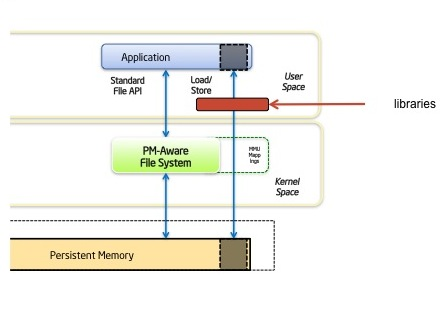
\includegraphics[scale=0.75]{figures/nvml-arch.jpg}
    \caption{System hierarchy indicating the position of NVML in red \cite{intel2014nvml}}
    \label{fig:nvml}
\end{figure}

Another discussed approach to manage NVRAM is through designated file systems
\cite{oukid2017data, andrei2017sap}. File systems provide a well-known and
suitable abstraction for non-volatile storage. In order to enable regular memory
access in a load-store manner, individual files can be mapped into virtual
memory. However, traditional file systems are not directly well-suited for use
with NVRAM. One reason is that most operating systems provide a page cache which
is used by file systems to defer expensive disk IO. In the case of NVRAM, page
caches may be no longer needed, as updates to NVRAM incur far less latency
compared to other non-volatile memories. In this regard, page caches even add
overhead instead of mitigating it. Apart from that, they add a level of
indirection which makes writes to NVRAM more likely to be torn by failures.
Also, traditional file systems are usually designed for block-oriented devices
which may no longer be the best option. Therefore, several NVRAM-aware file
systems have been proposed \cite{condit2009better, wu2011scmfs,
dulloor2014system, xu2016nova}. The key feature of these file systems is a
zero-copy mechanism by circumventing page caches. This enables true store-load
semantics for memory-mapped files. Other aspects include attempts to leverage
the byte-addressable nature of NVRAM and crash-related consistency issues.

Unfortunately, as of this writing there is no evident consensus regarding the
programming model to use for NVRAM \cite{boehm2016persistence}. Still,
middlewares such as NVML appear to be gaining the upper hand
\cite{oukid2017data, volos2017whisper, malinowski2017using, andrei2017sap}.

\paragraph{Consistency}

A notorious problem with NVRAM is consistency in case of crashes
\cite{condit2009better, dulloor2014system, oukid2017data}. Due to the complex
nature of this subject, further discussion is deferred to the next section.

\section{Preserving Consistency}

As pointed out earlier, the consistency of data stored in NVRAM is vulnerable to
crashes or power failures. Since NVRAM is directly attached to the processor
memory interface, there is no need to use techniques such as DMA to transfer a
modified page to external storage. This also means that a memory operation
solely relies on the CPU which usually gives no confirmation when that operation
completes. In this context, there are two major issues that threaten the
consistency of data written to NVRAM, namely out-of-order execution and deferred
write-back.

\paragraph{Out-Of-Order Execution}

When executing a program, processors fetch instructions on a consecutive manner.
Some instructions may inflict minimal latency, while others such as load
operations may delay further execution for hundreds of cycles. In an attempt to
optimize instruction throughput, individual instructions may be reordered. While
compilers may statically define promising orders, processors are able to reorder
instructions at runtime. This enables processors to optimize resource
utilization and hide latencies of time-consuming instructions. However, only
reorderings that do not violate data dependencies between instructions are
possible. While processors do prevent such conflicts, there are dependencies
that cannot be observed. For example, in order to mark a chunk of data as
durable in NVRAM, one might store a designated flag immediately after the
operation completed. With out-of-order execution it is possible that the flag is
written before the payload. This can lead to severe inconsistencies especially
when a crash prevents the chunk from being written.

A common method to counter this issue is to enforce memory order with memory
barriers (also fences) \cite{dulloor2014system, schwalb2016hyrise,
oukid2017data}. A memory barrier prevents the CPU from proceeding until all
prior memory operations have completed. Although a barrier does not directly
order its preceding instructions, it can be used to impose an order on separate
sequences of instructions. An example for a memory barrier is \code{sfence} on
x86 architectures. While this approach solves the initial problem, it has a
notable drawback. Memory barriers defeat the purpose of out-of-order execution.
As a result, CPU pipelines are likely to stall, hence reducing resource
utilization. Furthermore, store buffers are flushed leading to higher latencies
when accessing data of deferred store operations. Therefore, barriers can have
significant impact on runtime performance, unless used judiciously. With
\emph{epoch barriers} a similar approach has been proposed to address both order
and durability issues \cite{condit2009better}.

\paragraph{Deferred Write-Back}

In many modern processor architectures store operations may not  be immediately
lead to an update in main memory. This behaviour can be caused by intermediary
buffers such as memory order buffers, caches, and memory controller buffers.
While their individual purpose may vary, they all defer memory write-back
operations. This is a known vulnerability for consistency in NVRAM as the
mentioned buffers are volatile and deferred stores may be lost when power fails
\cite{condit2009better, oukid2017data}. In order to preserve consistency, it is
necessary to force write-back in all of these cases.

\begin{figure}[!ht]
    \centering
    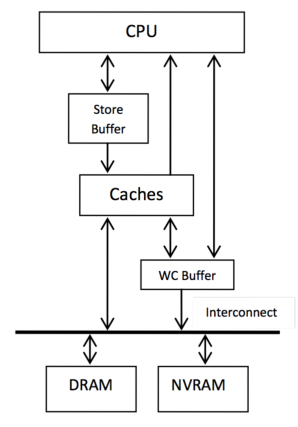
\includegraphics[scale=0.75]{figures/nvram-memory-subsystem.pdf}
    \caption{Architecture of memory subsystem \cite{bhandari2012implications}}
    \label{fig:nvml}
\end{figure}

% memory order buffers

In conjunction with instruction scheduling and cache coherency protocols a
memory order buffer may be present. It holds all loads and stores, with the
exception of non-temporal operations. In order to prevent a deferred write-back
through memory order buffers, their store buffers must be flushed. On x86
architectures this can be achieved with a store fence operation such as
\code{sfence}. As mentioned above, memory barriers carry a considerable
overhead. However, if memory barriers are already used for enforcing program
order, then flushing store buffers is a desirable side effect and incurs no
overhead.

% caches

Processor caches help avoid access latencies and reduce memory bus traffic for
frequently used data. A possible exception are non-temporal stores and data
chunks marked as uncacheable. Similar to memory order buffers, caches are
volatile so an abrupt power failure may lead to lost updates. The issue with
this is not that updates are lost but that it is unclear which updates are lost,
if any. The reason for this circumstance is the cache eviction policy trying to
compensate for typically narrow cache volume. Depending on policy, cache
content, and system load, a modified chunk may or may not be flushed to main
memory. An example of an application scenario where such behaviour is
unacceptable is transactions. Imagine an updating transaction $t1$ that commits
but is not evicted from cache. Then a transaction $t2$ based on the result of
$t1$ commits and gets evicted from cache. If the system crashes at this point,
$t2$'s result will be durable while $t1$'s initial update is lost.

\todo[inline]{graphic example?}

\begin{lstlisting}
T1: r(A) w(A) c*   -- Cache ---------------------- (crash)
T2: -------------- r(A) w(B) c -- Cache -- RAM --- (crash)
\end{lstlisting}

An approach to prevent such inconsistencies is to disable caching for selected
memory regions but that could introduce considerable overhead for frequently
used data. A more popular approach is to evict cache lines programmatically
whenever necessary \cite{condit2009better, dulloor2014system, oukid2017data}. On
x86 architectures this can be done with the \code{clflush} or \code{clflushopt}
instructions. However, the problem with a simple cache line flush such as
\code{clflush} is that making a cache line durable may not always mean that is
should be evicted. In this regard, \code{clwb} compensates for this matter by
retaining the designated cache line \cite{kolli2016high}. Unfortunately, at the
time of this writing there is no evidence of a processor to implement this
instruction.

% memory controller queues

Once a cache line is flushed, it is propagated to the memory controller where it
is buffered in a write-back queue before being written onto the device. Again,
the problem is that such a buffer is usually volatile. This means that a power
failure could lead to lost updates to NVRAM. Even though residual power in DRAM
has been shown to be substantial, there is no reliable way to ensure a full
buffer flush \cite{halderman2008lest}. This circumstance has given rise to many
discussions in the past \cite{condit2009better, dulloor2014system,
kolli2016high}. Some authors proposed a designated instruction for flushing
write-back queues. An example is the meanwhile deprecated \code{pcommit},
formerly known as \code{pm\_wbarrier} \cite{dulloor2014system, oukid2015instant,
schwalb2015nvm_malloc, volos2017whisper}. Others have developed more general
mechanisms for preserving consistency in NVRAM that also address this issue
\cite{condit2009better, pelley2014memory}. The current state of affairs is
that platforms must provide a feature called ADR \cite{volos2017whisper}. It
works by exploiting the fact that even in case of a power failure there is
sufficient power to flush the write buffers of all memory controllers. For this
to work, the power supply unit has to detect a power failure and issue a signal
to all memory controllers. As a result, neither programmers nor processors need to worry about memory controller queues while no overhead is incurred.

\paragraph{Summary}

\begin{itemize}
    \item this chapter touched several aspects of NVRAM research: ...
    \item the most ingriguing use case in conventional systems are MMDB/KVS
    \item in accordance with recent research, it is assumed that NVRAM complements DRAM instead of replacing it
    \item through hybrid mem arch benefits of both techs can be leveraged
    \item in context of MMDB it seems reasonable to refrain from using conventional non-volatile storage
    \item with PCM a promising technology nears commercial release
    \item concerning integration, it is very likely that NVRAM will be packaged as NVDIMM, so integration patterns are likely to remain largely the same
    \item consistency across crashes is still a prominent issue with NVRAM
    \item however, recent research suggests that a combination of memory barriers, cacheline flushes, and ADR provides a viable solution
    \item still, an open question is the programming model used with NVRAM
    \item as a result, a number of programming models have emerged
    \item in practice, programmers still need to meticulously manage non-volatile data (assignment policy, datastructure recovery, consistency)
    \item but programming models are beyond the scope of this work
\end{itemize}
